\documentclass[12pt,a4paper]{article}

% ─── Page Layout ───────────────────────────────────────────────────────────────
\usepackage[a4paper, margin=0.8in, headheight=14pt]{geometry}

% ─── Fonts (XeLaTeX) ───────────────────────────────────────────────────────────
\usepackage{fontspec}
\usepackage{unicode-math}
\setmainfont{TeX Gyre Pagella}
\setmonofont[Scale=0.88]{TeX Gyre Cursor}
\setmathfont{Latin Modern Math}

% ─── Packages ──────────────────────────────────────────────────────────────────
\usepackage{xcolor}
\usepackage{colortbl}
\usepackage{titlesec}
\usepackage{enumitem}
\usepackage{tabularx}
\usepackage{booktabs}
\usepackage{array}
\usepackage{amsmath}
\usepackage{tikz}
\usetikzlibrary{shapes.geometric, arrows.meta, positioning, calc, fit, decorations.pathreplacing, decorations.pathmorphing}
\usepackage{tcolorbox}
\tcbuselibrary{skins, breakable}
\usepackage{hyperref}
\usepackage{fancyhdr}
\usepackage{graphicx}
\usepackage{microtype}
\hyphenpenalty=10000
\exhyphenpenalty=10000
\sloppy
\usepackage{caption}
\usepackage{setspace}
\usepackage{multirow}
\usepackage{tocloft}

% ─── Q&A helper ────────────────────────────────────────────────────────────────
\newcommand{\Q}[1]{\textbf{#1}\par\noindent\ignorespaces}

% ─── Colour Palette ────────────────────────────────────────────────────────────
\definecolor{myred}{RGB}{196,30,58}
\definecolor{mydark}{RGB}{30,30,50}
\definecolor{mygreen}{RGB}{14,120,80}
\definecolor{myteal}{RGB}{0,130,140}
\definecolor{myamber}{RGB}{180,100,0}
\definecolor{mypurple}{RGB}{100,30,160}
\definecolor{mygray}{RGB}{246,247,249}
\definecolor{mgframe}{RGB}{180,185,200}
\definecolor{watermark}{RGB}{145,150,170}
\definecolor{hdrred}{RGB}{250,232,235}
\definecolor{hdrgreen}{RGB}{220,244,233}
\definecolor{hdrteal}{RGB}{220,242,244}
\definecolor{hdramber}{RGB}{253,242,215}
\definecolor{hdrpurple}{RGB}{238,228,255}
\definecolor{hdrgray}{RGB}{238,240,245}
\definecolor{rowalt}{RGB}{250,251,253}

% ─── Section Formatting ────────────────────────────────────────────────────────
\titleformat{\section}
  {\large\bfseries\color{myred}}{\thesection.}{0.5em}{}
  [\vspace{1pt}{\color{myred}\rule{\linewidth}{0.8pt}}]
\titleformat{\subsection}
  {\normalsize\bfseries\color{myteal}}{\thesubsection}{0.5em}{}
\titlespacing*{\section}{0pt}{18pt}{7pt}
\titlespacing*{\subsection}{0pt}{11pt}{4pt}

% ─── Paragraph ─────────────────────────────────────────────────────────────────
\setlength{\parindent}{0pt}
\setlength{\parskip}{4pt}

% ─── TOC Styling ───────────────────────────────────────────────────────────────
\renewcommand{\cfttoctitlefont}{\large\bfseries\color{myred}}
\renewcommand{\cftaftertoctitle}{\par\noindent{\color{myred}\rule{\linewidth}{0.8pt}}}
\setlength{\cftbeforetoctitleskip}{0pt}
\setlength{\cftaftertoctitleskip}{6pt}
\renewcommand{\cftsecfont}{\normalsize\bfseries\color{mydark}}
\renewcommand{\cftsecpagefont}{\normalsize\bfseries\color{mydark}}
\renewcommand{\cftsecleader}{\cftdotfill{\cftdotsep}}
\setlength{\cftbeforesecskip}{7pt}
\renewcommand{\cftsubsecfont}{\small\color{mydark}}
\renewcommand{\cftsubsecpagefont}{\small\color{mydark}}
\setlength{\cftbeforesubsecskip}{3pt}
\setlength{\cftsubsecindent}{1.4em}

% ─── Table helpers ─────────────────────────────────────────────────────────────
\renewcommand{\arraystretch}{1.45}
\setlength{\tabcolsep}{6pt}
\arrayrulecolor{mydark}
\newcolumntype{B}[1]{>{\small\bfseries\raggedright\arraybackslash}m{#1}}
\newcolumntype{C}[1]{>{\centering\arraybackslash}m{#1}}
\newcolumntype{Y}{>{\small\raggedright\arraybackslash}X}
\renewcommand{\tabularxcolumn}[1]{m{#1}}

% ─── Header / Footer ───────────────────────────────────────────────────────────
\pagestyle{fancy}
\fancyhf{}
\fancyhead[L]{\small\color{myred}\textbf{OE-EC704A}\;\color{mydark}--- Web Technology}
\fancyhead[R]{\small\color{myteal}\textbf{Module 6 Notes}}
\fancyfoot[C]{\small\color{mydark}\thepage}
\fancyfoot[R]{\small\color{watermark}\textit{\copyright\ Biraj}}
\renewcommand{\headrulewidth}{0.5pt}
\renewcommand{\footrulewidth}{0.3pt}

% ─── Hyperref ──────────────────────────────────────────────────────────────────
\hypersetup{
  colorlinks=true, linkcolor=myteal, urlcolor=myteal,
  pdfauthor={Biraj Sarkar},
  pdftitle={OE-EC704A --- Module 6 Notes}
}

% ─── tcolorbox styles ──────────────────────────────────────────────────────────
\tcbset{
  tikzbox/.style={
    colback=mygray, colframe=mgframe, boxrule=0.6pt, arc=4pt,
    left=8pt, right=8pt, top=6pt, bottom=6pt,
    colbacktitle=mgframe, coltitle=mydark,
    fonttitle=\small\bfseries
  },
  defbox/.style={
    colback=hdrgreen, colframe=mygreen, boxrule=0.8pt, arc=4pt,
    left=9pt, right=9pt, top=6pt, bottom=6pt,
    colbacktitle=mygreen, coltitle=white,
    fonttitle=\small\bfseries
  },
  formulabox/.style={
    colback=hdrteal, colframe=myteal, boxrule=0.8pt, arc=4pt,
    left=9pt, right=9pt, top=7pt, bottom=7pt,
    colbacktitle=myteal, coltitle=white,
    fonttitle=\small\bfseries
  },
  examplebox/.style={
    colback=hdramber, colframe=myamber, boxrule=0.8pt, arc=4pt,
    left=9pt, right=9pt, top=6pt, bottom=6pt,
    colbacktitle=myamber, coltitle=white,
    fonttitle=\small\bfseries
  },
  masonbox/.style={
    colback=hdrpurple, colframe=mypurple, boxrule=0.8pt, arc=4pt,
    left=9pt, right=9pt, top=6pt, bottom=6pt,
    colbacktitle=mypurple, coltitle=white,
    fonttitle=\small\bfseries
  },
  exambox/.style={
    colback=hdrpurple, colframe=mypurple, boxrule=1pt, arc=5pt,
    left=10pt, right=10pt, top=8pt, bottom=8pt,
    colbacktitle=mypurple, coltitle=white,
    fonttitle=\bfseries,
    breakable, title after break={\textbf{Frequently Asked / Viva Questions (contd.)}}}
}
\tcbset{breakable}

% ─── TikZ styles ───────────────────────────────────────────────────────────────
\tikzset{
  block/.style={rectangle, draw=myteal, fill=hdrteal,
    text width=2.5cm, align=center, minimum height=1.0cm,
    font=\small, rounded corners=3pt, line width=0.7pt},
  redblock/.style={rectangle, draw=myred, fill=hdrred,
    text width=2.5cm, align=center, minimum height=1.0cm,
    font=\small, rounded corners=3pt, line width=0.7pt},
  netnode/.style={rectangle, draw=myteal, fill=hdrteal,
    text width=1.8cm, align=center, minimum height=0.8cm,
    font=\small, rounded corners=3pt, line width=0.7pt},
  sumjunc/.style={circle, draw=myamber, fill=hdramber,
    minimum size=0.6cm, font=\small, line width=0.8pt},
  snode/.style={circle, draw=mypurple, fill=hdrpurple,
    minimum size=0.55cm, font=\footnotesize, line width=0.7pt},
  arrow/.style={-Stealth, thick, color=mydark},
  redarrow/.style={-Stealth, thick, color=myred},
  line/.style={thick, color=mydark}
}

% ═══════════════════════════════════════════════════════════════════════════════
\begin{document}
% ═══════════════════════════════════════════════════════════════════════════════

\begin{center}
  {\LARGE\bfseries\color{myred} OE-EC704A --- Web Technology}\\[5pt]
  {\normalsize\color{mydark} Semester VII \quad$\bullet$\quad 3L:0T:0P \quad$\bullet$\quad 3 Credits}\\[3pt]
  {\normalsize\color{myteal}\textbf{Module 6 Exam Notes: String Handling}}\\[3pt]
  {\small\color{mydark} CGEC \;$|$\; B.Tech ECE (2023--27) \;$|$\; \textit{Biraj Sarkar}}
\end{center}
\noindent{\color{myred}\rule{\linewidth}{1.5pt}}
\vspace{2pt}

\hypersetup{linkcolor=mydark}
\tableofcontents
\hypersetup{linkcolor=myteal}
\newpage

% ===============================================================================
\section{String Basics and Immutability}
% ===============================================================================

In Java, strings are represented by the \texttt{String} class inside the \texttt{java.lang} package. 

\begin{tcolorbox}[defbox, title={\textbf{String Immutability Concept}}]
Java String objects are \textbf{immutable}, meaning their values cannot be changed once they are created in memory. Any modification operation (like concatenation or case conversion) does not alter the original string; instead, it returns a reference to a completely new String object.
\end{tcolorbox}

\subsection{String Constant Pool (SCP)}
To save memory and increase performance, JVM maintains a special memory area inside the heap called the \textbf{String Constant Pool (SCP)}.
\begin{itemize}[leftmargin=*, itemsep=3.5pt]
  \item \textbf{Literal Allocation:} When a string is created using a literal (e.g., \texttt{String s1 = "Java";}), JVM first checks the SCP. If the string is already present, it returns the existing reference. Otherwise, it allocates a new string in the pool.
  \item \textbf{New Object Allocation:} Using the \texttt{new} keyword (e.g., \texttt{String s2 = new String("Java");}) bypasses pool checking and creates a new object in the general heap space, which references the literal value in the SCP.
\end{itemize}

\begin{tcolorbox}[tikzbox, title={String Memory References: General Heap vs. String Constant Pool (SCP)}]
\centering
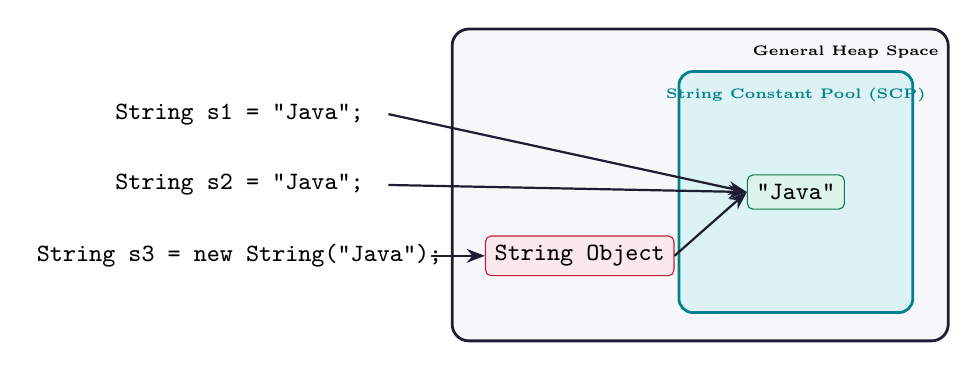
\begin{tikzpicture}[scale=0.9]
  % Stack variables
  \node (s1) at (-4, 2) {\small\texttt{String s1 = "Java";}};
  \node (s2) at (-4, 1) {\small\texttt{String s2 = "Java";}};
  \node (s3) at (-4, 0) {\small\texttt{String s3 = new String("Java");}};

  % General Heap Boundary
  \draw[draw=mydark, fill=mygray, line width=1pt, rounded corners=6pt] (-1,-1.2) rectangle (6,3.2);
  \node[anchor=north east, font=\tiny\bfseries] at (6,3.1) {General Heap Space};

  % SCP Boundary inside Heap
  \draw[draw=myteal, fill=hdrteal, line width=1pt, rounded corners=5pt] (2.2,-0.8) rectangle (5.5,2.6);
  \node[anchor=north, font=\tiny\bfseries, color=myteal] at (3.85,2.5) {String Constant Pool (SCP)};

  % String value inside SCP
  \node[draw=mygreen, fill=hdrgreen, rounded corners=2pt, font=\small\ttfamily] (java_literal) at (3.85, 0.9) {"Java"};

  % Heap object
  \node[draw=myred, fill=hdrred, rounded corners=2pt, font=\small\ttfamily] (heap_obj) at (0.8, 0) {String Object};

  % Connections
  \draw[arrow] (-1.9, 2) -- (java_literal.west);
  \draw[arrow] (-1.9, 1) -- (java_literal.west);
  \draw[arrow] (-1.3, 0) -- (heap_obj.west);
  \draw[arrow] (heap_obj.east) -- (java_literal.west);
\end{tikzpicture}
\end{tcolorbox}

% ===============================================================================
\section{String vs. StringBuffer}
% ===============================================================================

When a program performs frequent modifications to character sequences, using the immutable \texttt{String} class generates high amounts of garbage references. Java provides \texttt{StringBuffer} to resolve this.

\par\noindent
{\renewcommand{\arraystretch}{1.5}%
\begin{tabularx}{\linewidth}{|B{3.2cm}|Y|Y|}
\hline
\textbf{Metric} & \textbf{String Class} & \textbf{StringBuffer Class} \\
\hline
\textbf{Mutability} & Immutable (read-only). & Mutable (can modify in-place). \\
\hline
\textbf{Performance} & Slower for modifications. & Fast and memory efficient for loops. \\
\hline
\textbf{Thread Safety} & Naturally thread-safe. & Thread-safe (methods are synchronized). \\
\hline
\textbf{Memory Allocation} & Allocations inside the SCP or Heap. & Allocated strictly in the general Heap. \\
\hline
\end{tabularx}}

% ===============================================================================
\section{Constructors and Core Operations}
% ===============================================================================

\subsection{String Constructors}
\begin{itemize}[leftmargin=*, itemsep=3pt]
  \item \texttt{String()}: Initializes a newly created, empty String object.
  \item \texttt{String(char[] chars)}: Allocates a new String from an array of characters.
  \item \texttt{String(String original)}: Creates a copy of the argument string.
\end{itemize}

\subsection{Core String Operations}
\par\noindent
{\renewcommand{\arraystretch}{1.45}%
\begin{tabularx}{\linewidth}{|B{2.8cm}|B{4.5cm}|Y|}
\hline
\textbf{Operation} & \textbf{Method Signature} & \textbf{Functional Description} \\
\hline
\textbf{Extraction} & \texttt{char charAt(int index)} & Returns the character at the specified index. \\
                    & \texttt{int length()} & Returns the character count. \\
\hline
\textbf{Comparison} & \texttt{boolean equals(Object obj)} & Value-based comparison for character equality. \\
                    & \texttt{int compareTo(String another)} & Lexicographically compares two strings (returns difference). \\
\hline
\textbf{Searching}  & \texttt{int indexOf(String str)} & Returns the index of the first occurrence. \\
                    & \texttt{boolean contains(CharSequence s)} & Returns true if the string matches the pattern. \\
\hline
\textbf{Modifying}  & \texttt{String substring(int start, int end)} & Returns characters from start (incl.) to end (excl.). \\
                    & \texttt{String trim()} & Removes leading and trailing whitespace. \\
\hline
\end{tabularx}}

% ===============================================================================
\section{Utility Conversions}
% ===============================================================================

Java provides two major methods to perform conversions to strings:
\begin{itemize}[leftmargin=*, itemsep=3.5pt]
  \item \textbf{\texttt{toString()} Method:} Defined in the root \texttt{Object} class. Every Java class inherits it and can override it to provide a custom string representation of the object's fields.
  \item \textbf{\texttt{String.valueOf()} Static Method:} Overloaded methods to convert primitive data types (like \texttt{int}, \texttt{double}, \texttt{boolean}) or objects into string representations. If an object is passed, it returns \texttt{obj.toString()} or \texttt{"null"} safely if the reference is null.
\end{itemize}

% ===============================================================================
\section{StringBuffer Operations}
% ===============================================================================

\texttt{StringBuffer} maintains a growable character buffer, defaulting to 16 characters of extra capacity.
\begin{itemize}[leftmargin=*, itemsep=3.5pt]
  \item \textbf{\texttt{append()}:} Appends data to the end of the buffer.
  \item \textbf{\texttt{insert()}:} Inserts data at a specified index.
  \item \textbf{\texttt{reverse()}:} Reverses the sequence of characters in-place.
  \item \textbf{Capacity vs. Length:} \texttt{length()} returns the actual number of characters stored, while \texttt{capacity()} returns the total allocated buffer space.
\end{itemize}

\newpage
% ===============================================================================
\begin{center}
  {\large\bfseries\color{myred} Quick Revision --- Module 6}\\[3pt]
  {\small\color{mydark} String Handling $|$ OE-EC704A}
\end{center}
\noindent{\color{myred}\rule{\linewidth}{1.2pt}}
\vspace{4pt}

\begin{tcolorbox}[formulabox, title={\textbf{String \& StringBuffer Syntax}}]
{\renewcommand{\arraystretch}{1.3}%
\begin{tabularx}{\linewidth}{l Y}
\textbf{Operation} & \textbf{Syntax and Example Usage} \\
\hline
Literal Assignment & \texttt{String s1 = "Biraj"; // Allocated in SCP} \\
Object Constructor & \texttt{String s2 = new String("Biraj"); // Heap object reference} \\
Character Extraction & \texttt{char c = s1.charAt(2); // 'r'} \\
Substring Extraction & \texttt{String sub = s1.substring(1, 3); // "ir"} \\
\hline
\textbf{StringBuffer Operations} & \textbf{Mutable buffer syntax} \\
\hline
Declaration & \texttt{StringBuffer sb = new StringBuffer("CGE");} \\
Append Operation & \texttt{sb.append("C"); // sb becomes "CGEC"} \\
Insert Operation & \texttt{sb.insert(3, "-"); // sb becomes "CGE-C"} \\
In-place Reverse & \texttt{sb.reverse(); // sb becomes "C-EGC"} \\
\end{tabularx}}
\end{tcolorbox}

\begin{tcolorbox}[defbox, title={\textbf{One-Line Definitions}}]
\begin{itemize}[leftmargin=*, itemsep=2pt]
  \item \textbf{Immutability:} State constraint preventing modification of heap values after initial allocation.
  \item \textbf{String Constant Pool:} A cached region in Java heap memory storing unique string literals.
  \item \textbf{StringBuffer:} A thread-safe, synchronized, mutable character sequence class.
  \item \textbf{StringBuilder:} A non-synchronized, fast, mutable character sequence class.
  \item \textbf{equals():} Overridden method in String checking value-based character equality.
  \item \textbf{== Operator:} Operator checking whether two reference variables point to the same memory address.
  \item \textbf{valueOf():} Static String utility method converting primitives and objects to strings.
  \item \textbf{toString():} Standard Object method returning class representation details as a String.
\end{itemize}
\tcbset{after={\color{black}}}
\end{tcolorbox}

\begin{tcolorbox}[exambox, title={\textbf{Frequently Asked / Viva Questions}}]
\begin{enumerate}[leftmargin=*, label=\textbf{Q\arabic*.}, itemsep=5pt]
  \item \Q{Why are String objects immutable in Java?}
        To enable String Constant Pool caching (saving heap memory), ensure thread-safety, and prevent security vulnerabilities (since connection strings and file paths cannot be altered).
        
  \item \Q{What is the difference between \texttt{equals()} and \texttt{==} when comparing Strings?}
        \texttt{==} compares reference equality (whether variables point to the exact same object reference). The \texttt{equals()} method checks value equality (whether character sequences are identical).
        
  \item \Q{How many objects are created in the statement: \texttt{String s = new String("Hello");}?}
        Two objects. One literal object is placed in the String Constant Pool (if not already present), and a second String object is created in the general heap space.
        
  \item \Q{What does the method \texttt{intern()} do?}
        It returns the canonical representation of the string from the String Constant Pool. If the pool already contains the string, it returns its reference; otherwise, it adds the string to the pool and returns the reference.
        
  \item \Q{What is the difference between \texttt{StringBuffer} and \texttt{StringBuilder}?}
        Both are mutable classes. \texttt{StringBuffer} is thread-safe and has synchronized methods, causing high performance overhead. \texttt{StringBuilder} is not synchronized, making it faster and preferred for single-threaded applications.
        
  \item \Q{What is the default capacity of a \texttt{StringBuffer}? How does it increase?}
        The default initial capacity is 16. When the buffer capacity is exceeded, it grows automatically using the formula: $\text{New Capacity} = (\text{Old Capacity} \times 2) + 2$.
        
  \item \Q{Can we override the static method \texttt{valueOf()} in custom classes?}
        No. Static methods belong to the class scope and are resolved statically during compilation. They cannot be overridden in subclasses. Custom classes override \texttt{toString()} instead.
        
  \item \Q{What does the method \texttt{compareTo()} return?}
        It returns $0$ if strings are equal, a negative integer if the current string is lexicographically smaller than the argument, and a positive integer if it is larger.
        
  \item \Q{Why does \texttt{System.out.println(obj)} invoke the \texttt{toString()} method?}
        The print streams implicitly check if the argument is an object. If yes, it calls \texttt{String.valueOf(obj)}, which internally invokes \texttt{obj.toString()} to get a printable string.
        
  \item \Q{What is the purpose of the \texttt{trim()} method in the String class?}
        It returns a copy of the string with all leading and trailing whitespaces (characters with Unicode code point less than or equal to \texttt{'U+0020'}) removed.
\end{enumerate}
\end{tcolorbox}

\begin{tcolorbox}[tikzbox, title={Comparison: String vs. StringBuffer vs. StringBuilder}]
\centering
{\renewcommand{\arraystretch}{1.45}%
\begin{tabularx}{\linewidth}{|B{2.8cm}|Y|Y|Y|}
\hline
\textbf{Metric} & \textbf{String} & \textbf{StringBuffer} & \textbf{StringBuilder} \\
\hline
\textbf{Mutability} & Immutable. & Mutable. & Mutable. \\
\hline
\textbf{Thread Safety} & Yes (due to immutability). & Yes (synchronized methods). & No (non-synchronized). \\
\hline
\textbf{Performance} & Slowest for edits. & Slower (lock overhead). & Fastest. \\
\hline
\textbf{Introduced in} & Java 1.0 & Java 1.0 & Java 1.5 \\
\hline
\end{tabularx}}
\tcbset{after={\color{black}}}
\end{tcolorbox}

\end{document}
